\documentclass{article}
\usepackage{graphicx}
\usepackage{imakeidx}
\makeindex
\usepackage[utf8]{inputenc}
\usepackage[document]{ragged2e}
\usepackage{graphicx}

\renewcommand{\contentsname}{Indice}
\begin{document}
	\begin{centering}
    \vspace*{0.5 cm}
    \textsc{\LARGE Universidade do Minho}\\[2.0 cm]	% University Name
	\textsc{\LARGE Engenharia Informática}\\[1 cm]				% Course Code
	\textsc{\large 21/22}\\[0.5 cm]				% Course Name
	\rule{\linewidth}{0.2 mm} \\[0.4 cm]
	{ \huge \bfseries Redes - TP3}
	\rule{\linewidth}{0.2 mm} \\[1.5 cm]
		\begin{minipage}{0.4\textwidth}
		\begin{flushright}\large
		\begin{raggedright}
		Afonso Amorim A97569\par
		Luís Ferreira A95111\par
		Pedro Dantas  A97396\par
		\end{raggedright}
		\end{flushright}
	\end{minipage}
	\end{centering}
\clearpage
\tableofcontents
\cleardoublepage

\section{Captura e análise de Tramas Ethernet}\vspace{0.5cm}
\textbf{Exercício 1}

\vspace{0.5cm}
\begin{center}
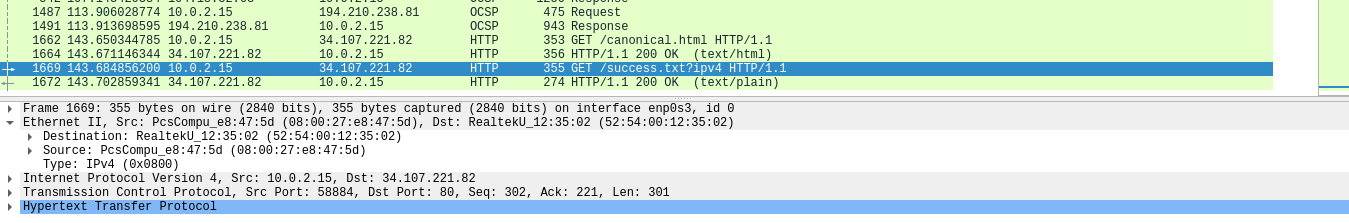
\includegraphics[width = 12cm]{1.png}

\caption{Fig. 1}
\end{center}

\vspace{0.5cm}
\textbf{Anote os endereços MAC de origem e de destino da trama capturada.}\par\vspace{0.35cm}
Endereço MAC de origem: \textbf{08:00:27:e8:47:5d}

Endereço MAC de destino: \textbf{52:54:00:12:35:02}

\vspace{0.5cm}
{\textbf{Exercício 2}}\vspace{0.5cm}

\textbf{Identifique a que sistemas se referem. Justifique.}\vspace{0.35cm}

\hspace{0.5cm}Relativamente à origem, o endereço físico é referente ao nosso computador (máquina utilizada). Por outro lado, o endereço de destino refere-se ao \textit{router} com o qual a nossa máquina está a comunicar.

\vspace{0.5cm}
{\textbf{Exercício 3}}\vspace{0.5cm}

\textbf{Qual o valor hexadecimal do campo \textit{Type} da trama \textit{Ethernet}? O que significa?}\vspace{0.35cm}

\hspace{0.5cm}Como se pode verificar pela figura 1, o \textit{Type} é (0x800), pelo que concluimos que a camada superior está a usar um protocolo IPv4.

\vspace{0.5cm}
{\textbf{Exercício 4}}\vspace{0.5cm}

\textbf{Quantos \textit{bytes} são usados no encapsulamento protocolar, i.e. desde o início da trama até ao início dos dados do nível
aplicacional (\textit{Application Data Protocol: http-over-tls})? Calcule e indique, em percentagem, a sobrecarga (\textit{overhead})
introduzida pela pilha protocolar.}

\clearpage
{\textbf{Exercício 5}}\vspace{0.5cm}

\textbf{Qual é o endereço \textit{Ethernet} da fonte? A que sistema de rede corresponde? Justifique.}\vspace{0.35cm}

\hspace{0.5cm}Tendo em conta a figura 1, podemos verificar que o endereço \textit{Ethernet} da fonte é (52:54:00:12:35:02), correspondente ao endereço físico do \textit{router} que está a ser acedido pela nossa máquina.

\vspace{0.5cm}
{\textbf{Exercício 6}}\vspace{0.5cm}

\vspace{0.5cm}
\begin{center}
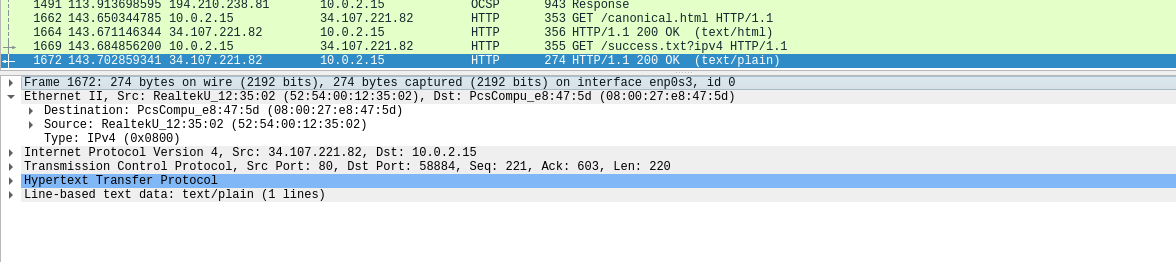
\includegraphics[width = 12cm]{4.png}

\caption{Fig. 2}
\end{center}

\vspace{0.5cm}

\textbf{Qual é o endereço MAC do destino? A que sistema corresponde?}\vspace{0.35cm}

\hspace{0.5cm}Tendo em conta a figura 2, verificamos que o endereço MAC do destino é (08:00:27:e8:47:5d), correspondente ao endereço físico da nossa máquina.

\vspace{0.5cm}
{\textbf{Exercício 7}}\vspace{0.5cm}

\textbf{Atendendo ao conceito de desencapsulamento protocolar, identifique os vários protocolos contidos na trama recebida.}\vspace{0.35cm}

\hspace{0.5cm}Os protocolos TCP (\textit{Tansmission Control Protocol}), IPv4 (\textit{Internet Protocol Version 4}), HTTP (\textit{Hypertext Transfer Protocol}) e \textit{Ethernet}.

\vspace{0.5cm}
\clearpage

\section{Protocolo ARP }\vspace{0.5cm}

\textbf{Exercício 8}

\vspace{0.5cm}
\begin{center}
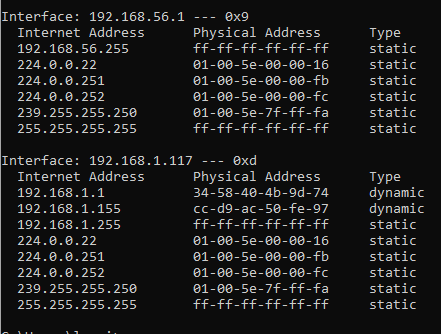
\includegraphics[width = 12cm]{2.png}

\caption{Fig. 3}
\end{center}

\textbf{Observe o conteúdo da tabela ARP. Diga o que significa cada uma das colunas.}\vspace{0.35cm}

\hspace{0.5cm}Como podemos observar na figura 3, a primeira coluna corresponde aos endereços IP, enquanto a segunda corresponde aos endereços MAC.

\vspace{0.5cm}
\clearpage
\textbf{Exercício 9}\vspace{0.5cm}

\textbf{Qual é o valor hexadecimal dos endereços origem e destino na trama Ethernet que contém a mensagem com o pedido ARP (\textit{ARP Request})? Como interpreta e justifica o endereço destino usado?}

\vspace{0.5cm}
\begin{center}
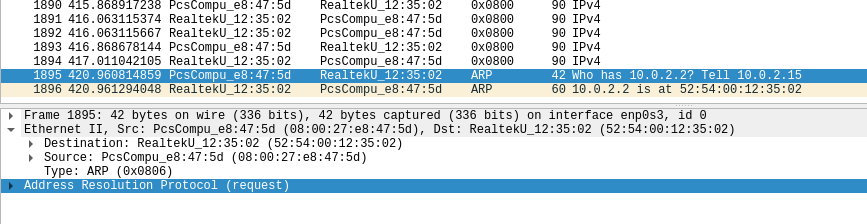
\includegraphics[width = 12cm]{3.png}

\caption{Fig. 4}
\end{center}

O valor do endereço origem é 08:00:27:e8:47:5d, enquanto o do destino é ff:ff:ff:ff:ff:ff. Este último pode ser justificado pelo facto de, na nossa tabela arp, o valor do endereço MAC não estar associado ao endereço IP para o qual o \textit{ping} é enviado. Desta forma, é necessário enviar uma mensagem para todos os dispositivos na rede de modo a que o dispositivo pretendido possa responder e, assim, guardar o valor do endereço MAC. Para isto é utilizado o endereço de Broadcast ff:ff:ff:ff:ff:ff.


\vspace{0.5cm}
\textbf{Exercício 10}\vspace{0.5cm}

\textbf{Qual o valor hexadecimal do campo tipo da trama \textit{Ethernet}? O que indica?}\vspace{0.35cm}

\hspace{0.5cm}Tendo em conta a figura x, podemos verificar que o valor hexadecimal do campo tipo da trama \textit{Ethernet} é 0x0806, o que nos indica que a camada acima está a utilizar o protocolo ARP.

\vspace{0.5cm}
\textbf{Exercício 11}\vspace{0.5cm}

\textbf{Como pode confirmar que se trata efetivamente de um pedido ARP? Identifique que tipo de endereços estão contidos na mensagem ARP? Que conclui?}\vspace{0.35cm}

\hspace{0.5cm}É possível verificar se se trata ou não de um pedido ARP através da análise do protocolo utilizado que, neste caso, é de facto um protocolo ARP, dado por 0x0806. Uma mensagem ARP contém tanto endereços IP como endereços MAC, pelo que podemos concluir que o protocolo ARP realiza a conversão de um endereço IP para um endereço MAC da respetiva interface ativa.

\vspace{0.5cm}
\textbf{Exercício 12}\vspace{0.5cm}

\textbf{Explicite que tipo de pedido ou pergunta é feita pelo \textit{host} de origem.}\vspace{0.35cm}

\hspace{0.5cm}Tendo em conta que a nossa tabela arp não possui uma associação entre o endereço IP para o qual é enviado um ping e o seu respetivo endereço MAC, envia-se uma mensagem ARP para todos os dispositivos na rede de modo a que, caso o endereço IP pretendido receba esta mesma mensagem, seja possível responder com o seu endereço MAC.


\vspace{0.5cm}
\textbf{Exercício 13}\vspace{0.5cm}

\begin{center}
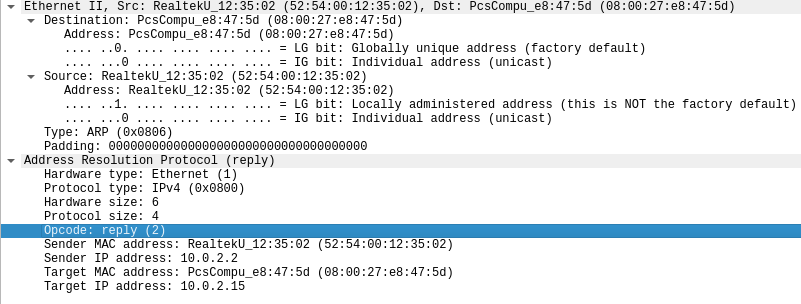
\includegraphics[width = 12cm]{5.png}

\caption{Fig. 5}
\end{center}

\vspace{0.5cm}
\begin{center}
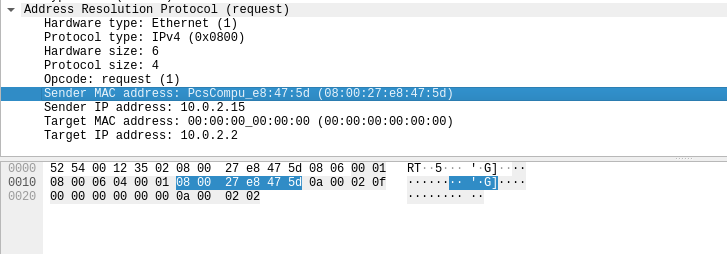
\includegraphics[width = 12cm]{6.png}

\caption{Fig. 6}
\end{center}

\vspace{0.5cm}

\textbf{Alínea (A)}

\textbf{Qual o valor do campo ARP opcode? O que especifica?}\vspace{0.35cm}

\hspace{0.5cm}O valor do campo ARP opcode é 2, pelo que podemos concluir que é a \textit{reply} (como indicado na figura 5) a uma mensagem de \textit{request} efetuada anteriormente. Nesta \textit{reply} será enviado o endereço MAC.\vspace{0.5cm}

\textbf{Alínea (B)}

\textbf{Em que campo da mensagem ARP está a resposta ao pedido ARP?}\vspace{0.35cm}

\hspace{0.5cm}A resposta ao pedido ARP encontra-se entre 23 - 28 \textit{bytes}, como podemos verificar através da figura 6. Esta informação pode ser obtida através do \textit{Sender MAC Address}.

\vspace{0.5cm}
\textbf{Exercício 14}\vspace{0.5cm}

\textbf{Na situação em que efetua um \textit{ping} a outro \textit{host}, assuma que este está diretamente ligado ao mesmo \textit{router}, mas noutra
subrede, e que todas as tabelas ARP se encontram inicialmente vazias. Esboce um diagrama em que indique claramente,
e de forma cronológica, todas as mensagens ARP e ICMP trocadas, até à recepção da resposta ICMP do \textit{host} destino.}


\vspace{0.5cm}

\section{Domínios de colisão}\vspace{0.5cm}

\textbf{Exercício 15}\vspace{0.5cm}

\textbf{Através da opção \textit{tcpdump} verifique e compare como flui o tráfego nas diversas interfaces do dispositivo de interligação
no departamento A (\textit{LAN} partilhada) e no departamento B (\textit{LAN} comutada) quando se gera tráfego intra-departamento (por
exemplo, fazendo ping \textit{IPaddr} da \textit{Bela} para \textit{Monstro}, da \textit{Jasmine} para o \textit{Alladin}, etc.) Que conclui?}

\vspace{2cm}

\textbf{Exercício 16}\vspace{0.5cm}

\textbf{Construa manualmente a tabela de comutação do \textit{switch} do Departamento B, atribuindo números de porta à sua escolha.}


\vspace{0.5cm}
\clearpage

\section{Conclusão}\vspace{0.5cm}

Após a realização do trabalho podemos concluir que obtivemos uma melhor compreensão em relação a tramas \textit{Ethernet} e ao protocolo ARP, que foram estudados nas duas primeiras fases. Para isto utilizamos o \textit{software} de captura e análise de tramas \textit{Wireshark}. Esta ferramenta foi essencial para diversos aspectos como: a verificação dos protocolos utilizados, o encapsulamento aquando da transferência de processos, o tipo de mensagem ARP, etc.
Foi também utilizado, indiretamente, o \textit{CORE}, sendo que não foram necessárias alterações em relação ao que foi feito num trabalho prático realizado anteriormente. 


\end{document}